%%%%%%%%%%%%%%%%%%%%%%%%%%%%%%%%%%%%%%%%%%%%%%%%%%%%%%%%%%%%%%%%%%%
% Sprint 3
% Team:
% Wolverine
% Members: 
% Eric Lee, Jacky Wu, Karthick Mani, 
% Eric Chang, Dexter Cheng, Peter Cheng
% Relative files:
% Team_Wolverine.tex, Team_Wolverine_Compile.tex, Library.bib, WolverineChart.png
% Note:    
% Do not compile this file compile Team_Wolverine_Compile.tex to get the pdf file instead.
%%%%%%%%%%%%%%%%%%%%%%%%%%%%%%%%%%%%%%%%%%%%%%%%%%%%%%%%%%%%%%%%%%%
	
\subsection*{Team Wolverine}
\label{Group}
	
Eric Lee, Jacky Wu, Karthick Mani, Eric Chang, Dexter Cheng, Peter Cheng
	
\subsection*{Create a data base of open access full text article}
\label{task1}

Goal for this subsection is to build up a database which downloads articles from open access databases using web crawler or web robot. And setting up a system that can allow the users to access the data in our database. I'd like to seperate this subsection into six features, then I'll give several suggestions based on each feature. 

\paragraph*{Feature 1 --Administrator}
\label{task1:part1}

In this part, the main consideration is the relationship between user and administrator. As an administrator's point, I'd like to give the best product to the consumer. On the other hand, users want to have convenient searching engine to get in touch with the knowledge. For this purpose, I'm pressure to show two suggestions for enhancing the relationship between users and producers. First, set up a popular-word-ranking system. When I search in something I don't know its name but know it in some specific area, such as stem cell in medical area. In this moment, the popular-word-ranking system will help me searching by giving me some keywords. Then, I would be easily to use this database. Of course, the popular-word-ranking system is based on users' searches and experts'suggestions to change the key words. So, the system can be trusted. 
	
Second, build up an area in the database and let user to change the area to what they want it to be. The idea is referenced from well-known media, Wikimedia. It's so called "personalized searching". By doing this, it would help user idealize the system to what they want and suggest administrator the service which clients really want. It would lead to a win-win situation.
	
\paragraph*{Feature 2 -- Web Crawler}
\label{task1:feature2}
	
The web crawler is a algorithm that has ability to quickly and accurately process and update a very large amount of data which are constantly being updated.\cite{Liu2012} It starts with a list of URLs to visit, called the seeds. As the crawler visits these URLs, it identifies all the hyperlinks in the page and adds them to the list of URLs to visit, called the crawl frontier. URLs from the frontier are recursively visited according to a set of policies. If the crawler is performing archiving of websites it copies and saves the information as it goes. The archives are usually stored in such a way they can be viewed, read and navigated as they were on the live web, but are preserved as �snapshots'.\cite{Du2013} We need to build up a web crawler to automatically visit a list of web page. Then find out which link in the page is valuable to download it into our database. 
	
\paragraph*{Feature 3 -- User account}
\label{task1:feature3}
	
In this part, the main issue is how to create a user account that can connect between user and database. But the more important thing is to make sure database will not collapse by user who is not allowed to access to core part of database.
To protect the database system security and privilege, this study introduces two methods for user account, principle of least privilege and role-based access control respectively. The principle of least privilege, also known as the principle of minimal privilege, means giving a user account only those those privileges which are essential to that users work \cite{PrincipleLeastPrivilege}. The role-based access control is a policy neutral access control mechanism defined around privileges and roles. It can implement discretionary access control (DAC) or mandatory access control (MAC). The role-based access control is very easy to do user assignments as the components of this policy, such as role-permissions, etc. That is why it sometimes referred to as role-based security \cite{RoleBasedAccessControl}. The information and resources would not in danger due to these two methods will filter user depend on their authority and only allow the legitimate user to access.	
To protect the database system security and privilege, this study introduces two methods for user account, principle of least privilege and role-based access control respectively. The principle of least privilege, also known as the principle of minimal privilege, means giving a user account only those those privileges which are essential to that user`s work \cite{PrincipleLeastPrivilege}. The role-based access control is a policy neutral access control mechanism defined around privileges and roles. It can implement discretionary access control (DAC) or mandatory access control (MAC). The role-based access control is very easy to do user assignments as the components of this policy, such as role-permissions, etc. That is why it sometimes referred to as role-based security \cite{RoleBasedAccessControl}. The information and resources would not in danger due to these two methods will filter user depend on their authority and only allow the legitimate user to access.
	
\paragraph*{Feature 4 -- User Interface}
\label{task1:feature4}
	
Understanding the types of visualizations people create by themselves for personal use. As part of this recent direction, we have studied a large collection of whiteboards in a research institution, where people make active use of combinations of words, diagrams and various types of visuals to help them further their thought processes. Our goal is to arrive at a better understanding of the nature of visuals that are created spontaneously during brainstorming, thinking, communicating, and general problem solving on whiteboards.\cite{Blascheck2016} We use the qualitative approaches of open coding, interviewing, and affinity diagramming to explore the use of recognizable and novel visuals, and the interplay between visualization and diagrammatic elements with words, numbers and labels. We discuss the potential implications of our findings on information visualization design. Combining the advantage of visual thinking new standard of data processing, that visual nature of computers can challenge the first generation of hackers, An icon is an image, picture, or symbol representing a concept.\cite{Szpunar2010}
	
\paragraph*{Feature 5 -- Data Storage and Search Methods}
\label{task1:feature5}

The organization of data inside a database management system(DBMS) and retrieval methods is based on the database storage structure such as tables and indexes. 
There are several types of database storage structure such as XML, a textual data format. 
This advantage is self-describing and flexible in organizing data.\cite{ISI:000253400700005}Several considerations of data storage include right space allocation techniques, data compression techniques (if necessary), security and encryption and the access path to retrieve the data. 
Therefore, DBMS software provides some method to optimize and  minimum storage space of a database.

\paragraph*{Feature 6 -- Database Management Systems}
\label{task1:feature6}
	
The relational database model was proposed by Edgar Codd in 1970, but because of the technological requirements it was not universal at that time. It was until 1980s that the first commercial relational database management systems began to appear. 
A database management system (DBMS) is a computer software application that interacts with the user, other applications, and the database itself to capture and analyze data. Well-known DBMSs include MySQL, PostgreSQL, Microsoft SQL Server, Oracle, Sybase and IBM DB2. 
Queries are the main way in which users retrieve information from a database. Most database management systems use a standard system called Structured Query Language (SQL) to query their tables. SQL is a structured form of English and resembles many programming languages, although most systems provide a graphical user-interface to generate the SQL code. And the most popular database systems since the 1980s have all supported the relational model as represented by the SQL language.\cite{Martinez-Cruz2011} hello	
	
\begin{figure*}[h]
	\begin{center}
		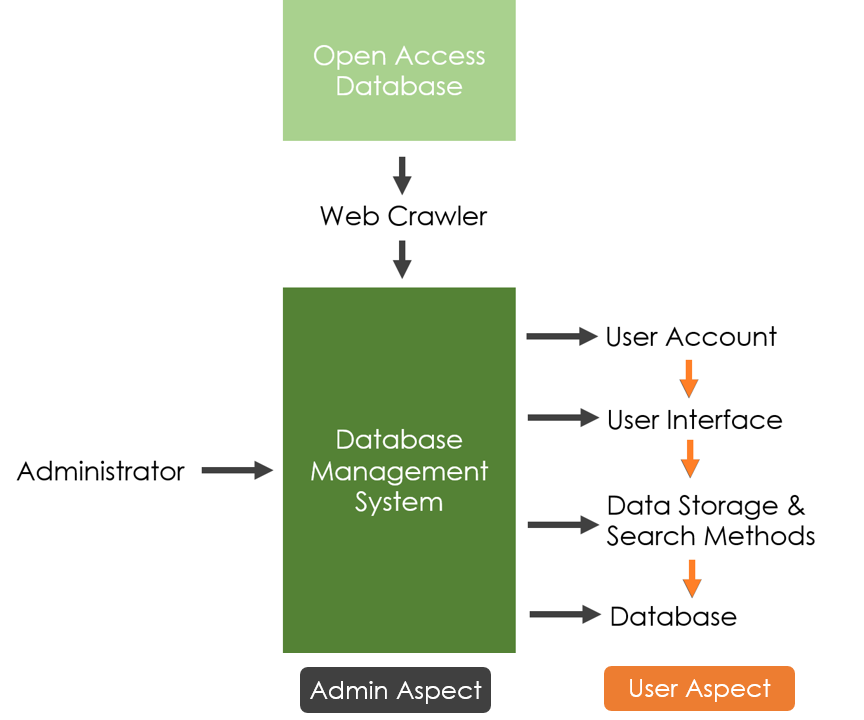
\includegraphics[scale=1.0]{WolverineChart}
	\end{center}
	\caption{Hierarchical overview}
\end{figure*}
\clearpage
